\documentclass[10pt]{article}
\usepackage{icmlko}

\icmlmeta{IP 파운데이션 월드모델}{56}{경계가 아니라 비탈이었다}{축 하나를 꺼 삼축 도메인을 열두 개 만들어 보니 절반만 고유 축이 도움된다 --- 그리고 갈리는 이유가 따로 있다}

\begin{document}

\twocolumn[
\icmlheader

\begin{abstract}
노트 55는 ``고유 축은 관측 축이 성분 수(둘)와 같을 때만 도움이 된다''고 하고
경계를 셋 근처에 그었다. 관측 축이 셋인 도메인이 없어 경계 위치를 몰랐으므로,
사축 도메인(도서 · 펀딩 · 웹툰)에서 축을 하나씩 꺼 삼축 상태를 열두 개 만들었다.
\textbf{6/12에서 고유 축이 도움된다.} 관측 축 둘이면 1/1, 셋이면 6/12, 넷이면
0/3, 다섯이면 0/2로 \textbf{단조 감소하는 비탈}이지 경계가 아니다. 그리고 삼축
안에서 무엇이 갈리는지 보였다 --- \textbf{끈 축을 고유 축이 대신할 수 있느냐}다.
웹툰에서 타깃 폭을 끄면 기준이 $+$0.3440에서 $+$0.2763으로 크게 떨어지는데
고유 축이 $+$0.0458로 가장 크게 회복한다. 웹툰 고유 축에 태그 수가 들어 있고
그것이 원래 타깃 폭이었기 때문이다. 반대로 웹툰 굿즈 규모를 끄면 $-$0.0530으로
가장 나쁘다 --- 고유 축에 참여 작가 수를 대신할 것이 없다. 부수로 확인된 것이
하나 더 있다. 축 하나를 끌 때 기준이 가장 크게 떨어지는 자리가 \textbf{타깃
폭}이다(세 도메인 모두). 노트 47이 배선 승리가 타깃 폭에 몰린다고 했다가
노트 48에서 우연으로 정정했는데, 다른 경로로 같은 자리가 다시 나온다.
\end{abstract}
]

\section{삼축 도메인을 만들었다}

노트 55의 한계 항목 첫 줄이 이랬다 --- ``관측 축이 셋인 도메인이 없어 경계
위치를 모른다.'' 만들면 된다. 사축 도메인 셋에서 축을 하나씩 꺼 열두 가지
삼축 상태를 얻었다.

기준은 그 삼축 상태 자체다. 즉 $\Delta\rho$ $=$ (삼축 $+$ 고유 축) $-$ (삼축).

\begin{figure}[t]
\centering
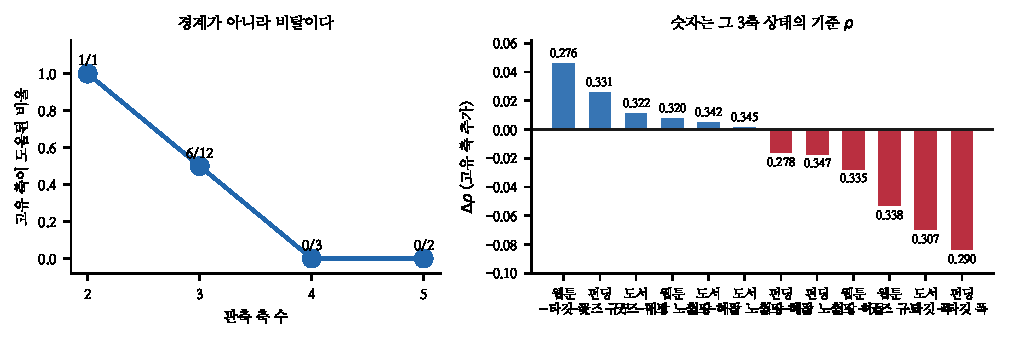
\includegraphics[width=\textwidth]{figs/slope.pdf}
\caption{왼쪽 --- 축 수별 도움 비율. 오른쪽 --- 삼축 열두 가지 각각.}
\end{figure}

\begin{table}[t]
\centering\tsize
\caption{관측 축 수와 고유 축의 효과.}
\begin{tabular}{lrr}
\toprule
관측 축 & 도움된 사례 & 비율 \\
\midrule
2 (게임) & 1/1 & 100\% \\
\textbf{3} (인위) & \textbf{6/12} & \textbf{50\%} \\
4 & 0/3 & 0\% \\
5 & 0/2 & 0\% \\
\bottomrule
\end{tabular}
\end{table}

\claimx{노트 55의 ``경계''를 정정한다. 축 수가 늘수록 고유 축의 도움이 단조로
줄어드는 비탈이며, 셋에서 절반이다. 넷 이상에서 0인 것은 그대로다.}{인위로
만든 삼축은 원래 삼축인 도메인과 다를 수 있다 --- 끈 축의 정보가 다른 축에
남아 있을 수 있다. 진짜 삼축 도메인이 들어오면 비율이 달라질 수 있다.}

\section{삼축 안에서 무엇이 갈리나}

\begin{table}[t]
\centering\tsize
\caption{삼축 열두 가지. 기준은 그 상태의 $\rho$다.}
\begin{tabular}{llrr}
\toprule
도메인 & 끈 축 & 기준 & $\Delta\rho$ \\
\midrule
웹툰 & 타깃 폭 & 0.2763 & \textbf{$+$0.0458} \\
펀딩 & 굿즈 규모 & 0.3312 & $+$0.0257 \\
도서 & 굿즈 규모 & 0.3221 & $+$0.0111 \\
웹툰 & 매장 노출도 & 0.3199 & $+$0.0074 \\
도서 & 입장 허들 & 0.3418 & $+$0.0048 \\
도서 & 매장 노출도 & 0.3454 & $+$0.0013 \\
\midrule
펀딩 & 입장 허들 & 0.2782 & $-$0.0159 \\
펀딩 & 매장 노출도 & 0.3471 & $-$0.0171 \\
웹툰 & 입장 허들 & 0.3354 & $-$0.0275 \\
웹툰 & 굿즈 규모 & 0.3375 & $-$0.0530 \\
도서 & 타깃 폭 & 0.3066 & $-$0.0695 \\
펀딩 & 타깃 폭 & 0.2899 & $-$0.0836 \\
\bottomrule
\end{tabular}
\end{table}

\claimx{삼축에서 고유 축이 도움되는지는 \textbf{끈 축을 고유 축이 대신할 수
있느냐}로 갈린다. 축 수는 여지를 만들 뿐이고 무엇으로 채우는지가 정한다.}
{웹툰 타깃 폭의 회복($+$0.0458)이 태그 수가 고유 축에 있어서라는 것은 사후
설명이다. 태그 수를 고유 축에서 빼고 다시 재면 검정된다.}

두 사례가 대조적이다.

\begin{itemize}[leftmargin=1.1em,itemsep=0.15em]
\item \textbf{웹툰 타깃 폭을 끔} --- 기준이 $+$0.2763까지 떨어지는데 고유 축이
      $+$0.0458 회복한다. 웹툰 고유 축에 태그 수가 있고 그것이 \emph{원래}
      타깃 폭이었다(노트 46에서 연령 등급을 밀어내고 채택된 것).
\item \textbf{웹툰 굿즈 규모를 끔} --- $-$0.0530으로 가장 나쁘다. 고유 축에
      참여 작가 수를 대신할 것이 없다(노트 48에서 채택된 축이다).
\end{itemize}

\section{타깃 폭이 또 나왔다}

부수로 확인된 것이 있다. 축 하나를 끌 때 기준이 가장 크게 떨어지는 자리가
세 도메인 모두 \textbf{타깃 폭}이다.

\begin{table}[t]
\centering\tsize
\caption{축 하나를 끌 때의 기준 $\rho$. 현행 전체는 $+$0.3440이다.}
\begin{tabular}{lrrrr}
\toprule
끈 축 & 도서 & 펀딩 & 웹툰 & 평균 \\
\midrule
\textbf{타깃 폭} & 0.3066 & 0.2899 & 0.2763 & \textbf{0.291} \\
굿즈 규모 & 0.3221 & 0.3312 & 0.3375 & 0.330 \\
입장 허들 & 0.3418 & 0.2782 & 0.3354 & 0.318 \\
매장 노출도 & 0.3454 & 0.3471 & 0.3199 & 0.337 \\
\bottomrule
\end{tabular}
\end{table}

노트 47은 배선 승리가 타깃 폭에 몰린다고 했다가 노트 48에서 셋째 승리가 굿즈
규모에서 나와 우연으로 정정했다. \textbf{여기서 완전히 다른 경로로 같은 자리가
다시 나온다} --- 배선을 바꾸는 것이 아니라 축을 끄는 것으로.

\claimx{타깃 폭은 다섯 축 중 대체 불가능성이 가장 큰 자리다. 끄면 세 도메인
모두에서 기준이 가장 크게 떨어진다.}{도메인 셋으로 본 것이고 팝업 · 아이돌 ·
게임에서는 안 했다. 특히 게임은 축이 둘뿐이라 끄면 하나가 되어 정렬이 불가능하다.}

노트 40에서 타깃 폭을 ``다섯 축 중 유일하게 상한을 재는 축''이라고 읽었는데
--- 매장 노출도 · 입장 허들 · 굿즈 규모는 정도의 문제인데 타깃 폭은 ``애초에
몇 명이 후보인가''를 잰다 --- 그 해석과 맞는다.

\section{한계}

\begin{itemize}[leftmargin=1.1em,itemsep=0.15em]
\item 인위로 만든 삼축이라 끈 축의 정보가 다른 축에 남아 있을 수 있다.
\item 열두 가지 각각에 짝지은 구간을 붙이지 않았다. $+$0.0013 같은 값은
      잡음일 것이다.
\item 각 도메인의 고유 축 후보를 내가 골랐으므로 ``대신할 수 있느냐''는 후보
      구성에 달려 있다.
\item 타깃 폭 결과는 도메인 셋에서만 봤다.
\item 웹툰이 1,112건까지 수집됐는데 이 실험은 900건 상태에서 돌렸다. 다시
      재야 한다.
\end{itemize}

\section{다음}

\begin{enumerate}[leftmargin=1.3em,itemsep=0.15em]
\item 웹툰 고유 축에서 태그 수를 빼고 타깃 폭 회복이 사라지는지 --- 이 노트의
      반증 조건.
\item 웹툰 전체 수집 완료 후 전면 재측정(1,112/3,973 진행 중).
\item 타깃 폭의 대체 불가능성을 팝업 · 아이돌에서도 확인한다.
\item 삼축 열두 가지 중 상위 몇에 구간을 붙인다.
\end{enumerate}

\vspace{0.6em}
\hrule height 0.3pt
\vspace{0.5em}
{\footnotesize
\textbf{참고문헌}\\[0.3em]
Jolliffe, I. T. (2002). \emph{Principal Component Analysis}, 2nd ed. Springer.\\[0.15em]
Guyon, I., Elisseeff, A. (2003). An introduction to variable and feature selection.
\emph{JMLR}, 3, 1157--1182.\\[0.15em]
Meredith, W. (1993). Measurement invariance, factor analysis and factorial
invariance. \emph{Psychometrika}, 58(4), 525--543.\\[0.15em]
Schönemann, P. H. (1966). A generalized solution of the orthogonal Procrustes
problem. \emph{Psychometrika}, 31(1), 1--10.\\[0.15em]
Ben-David, S. et al. (2010). A theory of learning from different domains.
\emph{Machine Learning}, 79(1--2), 151--175.
}

\end{document}
